\documentclass[draftspec]{ninemlspec}
\usepackage{microtype}
\usepackage{pbox}
\usepackage{multirow}
\usepackage{multicol}
\usepackage{float}
%% ============================================================================
%% Description:  Documentation for \lq\lq{}The NineML Specification Document\rq\rq{}
%% Authors: Thomas G. Close <tclose@oist.jp>, Ivan Raikov <raikov@oist.jp>, Andrew P. Davison <davison@unic.cnrs-gif.fr>
%% Organization: Okinawa Institute of Science and Technology Graduate University, Centre National de la Recherche Scientifique
%% Date created: October 2014  <---- should probably be some date in 2010, 2011 or so...
%% https://github.com/INCF/nineml/master/spec/specification.tex
%%
%% Copyright (C) 2014 Okinawa Institute of Science and Technology Graduate University, Centre National de la Recherche Scientifique
%%
%% ============================================================================

\newcommand{\incomplete}{\begin{center}\noindent{\Large\textcolor{incompletered}{\textbf{!! INCOMPLETE !!}}}\end{center}}

% Define misc. references
\newcommand{\identifier}{\typeDefRef{identifier\xspace}{sec:identifier}}
\newcommand{\URL}{\href{http://en.wikipedia.org/wiki/Uniform_resource_locator}{URL}\xspace}
\newcommand{\MathML}{\href{http://mathml.org}{MathML (http://mathml.org)}\xspace}

% Define Abstraction Layer element references

\newcommand{\Unit}{\defRef{\textbf{\class{Unit}}\xspace}{sec:Unit}}
\newcommand{\Dimension}{\defRef{\textbf{\class{Dimension}}\xspace}{sec:Dimension}}
\newcommand{\ComponentClass}{\defRef{\textbf{\class{ComponentClass}}\xspace}{sec:ComponentClass}}
\newcommand{\Dynamics}{\defRef{\defRef{\textbf{\class{Dynamics}}\xspace}{sec:Dynamics}}{sec:Dynamics}}
\newcommand{\Function}{\defRef{\textbf{\class{Function}}\xspace}{sec:Function}}
\newcommand{\BuiltInDistribution}{\defRef{\textbf{\class{BuiltInDistribution}}\xspace}{sec:BuiltInDistribution}}
\newcommand{\ConnectionRule}{\defRef{\textbf{\class{ConnectionRule}}\xspace}{sec:ConnectionRule}}
\newcommand{\ConnectCondition}{\defRef{\textbf{\class{ConnectCondition}}\xspace}{sec:ConnectCondition}}
\newcommand{\ExplicitConnections}{\defRef{\textbf{\class{ExplicitConnections}}\xspace}{sec:ExplicitConnections}}
\newcommand{\SourceIndices}{\defRef{\textbf{\class{SourceIndices}}\xspace}{sec:SourceIndices}}
\newcommand{\DestinationIndices}{\defRef{\textbf{\class{DestinationIndices}}\xspace}{sec:DestinationIndices}}
\newcommand{\SelectConnections}{\defRef{\textbf{\class{SelectConnections}}\xspace}{sec:SelectConnections}}
\newcommand{\Number}{\defRef{\textbf{\class{Number}}\xspace}{sec:Number}}
\newcommand{\Preference}{\defRef{\textbf{\class{Preference}}\xspace}{sec:Preference}}
\newcommand{\MathInline}{\defRef{\textbf{\class{MathInline}}\xspace}{sec:MathInline}}
\newcommand{\Piecewise}{\defRef{\textbf{\class{Piecewise}}\xspace}{sec:Piecewise}}
\newcommand{\Piece}{\defRef{\textbf{\class{Piece}}\xspace}{sec:Piece}}
\newcommand{\Expression}{\defRef{\textbf{\class{Expression}}\xspace}{sec:Expression}}
\newcommand{\Condition}{\defRef{\textbf{\class{Condition}}\xspace}{sec:Condition}}
\newcommand{\Otherwise}{\defRef{\textbf{\class{Otherwise}}\xspace}{sec:Otherwise}}
\newcommand{\StateVariable}{\defRef{\textbf{\class{StateVariable}}\xspace}{sec:StateVariable}}
\newcommand{\StateAssignment}{\defRef{\textbf{\class{StateAssignment}}\xspace}{sec:StateAssignment}}
\newcommand{\TimeDerivative}{\defRef{\textbf{\class{TimeDerivative}}\xspace}{sec:TimeDerivative}}
\newcommand{\Alias}{\defRef{\textbf{\class{Alias}}\xspace}{sec:Alias}}
\newcommand{\Constant}{\defRef{\textbf{\class{Constant}}\xspace}{sec:Constant}}
\newcommand{\RandomVariable}{\defRef{\textbf{\class{RandomVariable}}\xspace}{sec:RandomVariable}}
\newcommand{\Argument}{\defRef{\textbf{\class{Argument}}\xspace}{sec:Argument}}
\newcommand{\StandardLibrary}{\defRef{\textbf{\class{StandardLibrary}}\xspace}{sec:StandardLibrary}}
\newcommand{\Regime}{\defRef{\textbf{\class{Regime}}\xspace}{sec:Regime}}
\newcommand{\Trigger}{\defRef{\textbf{\class{Trigger}}\xspace}{sec:Trigger}}
\newcommand{\EventOut}{\defRef{\textbf{\class{EventOut}}\xspace}{sec:EventOut}}
\newcommand{\OnEvent}{\defRef{\textbf{\class{OnEvent}}\xspace}{sec:OnEvent}}
\newcommand{\OnCondition}{\defRef{\textbf{\class{OnCondition}}\xspace}{sec:OnCondition}}
\newcommand{\Parameter}{\defRef{\textbf{\class{Parameter}}\xspace}{sec:Parameter}}
\newcommand{\AnalogSendPort}{\defRef{\textbf{\class{AnalogSendPort}}\xspace}{sec:AnalogSendPort}}
\newcommand{\EventSendPort}{\defRef{\textbf{\class{EventSendPort}}\xspace}{sec:EventSendPort}}
\newcommand{\AnalogReceivePort}{\defRef{\textbf{\class{AnalogReceivePort}}\xspace}{sec:AnalogReceivePort}}
\newcommand{\AnalogReducePort}{\defRef{\textbf{\class{AnalogReducePort}}\xspace}{sec:AnalogReducePort}}
\newcommand{\AnalogArrayPort}{\defRef{\textbf{\class{AnalogArrayPort}}\xspace}{sec:AnalogArrayPort}}
\newcommand{\EventReceivePort}{\defRef{\textbf{\class{EventReceivePort}}\xspace}{sec:EventReceivePort}}
\newcommand{\PropertySendPort}{\defRef{\textbf{\class{PropertySendPort}}\xspace}{sec:PropertySendPort}}
\newcommand{\PropertyReceivePort}{\defRef{\textbf{\class{PropertyReceivePort}}\xspace}{sec:PropertyReceivePort}}
\newcommand{\IndexSendPort}{\defRef{\textbf{\class{IndexSendPort}}\xspace}{sec:IndexSendPort}}
\newcommand{\IndexReceivePort}{\defRef{\textbf{\class{IndexReceivePort}}\xspace}{sec:IndexReceivePort}}
\newcommand{\Annotations}{\defRef{\textbf{\class{Annotations}}\xspace}{sec:Annotations}}

% Define User Layer element references

\newcommand{\Component}{\defRef{\textbf{\class{Component}}\xspace}{sec:Component}}
\newcommand{\Property}{\defRef{\textbf{\class{Property}}\xspace}{sec:Property}}
\newcommand{\DerivedProperty}{\defRef{\textbf{\class{DerivedProperty}}\xspace}{sec:DerivedProperty}}
\newcommand{\Quantity}{\defRef{\textbf{\class{Quantity}}\xspace}{sec:Quantity}}
\newcommand{\SingleValue}{\defRef{\textbf{\class{SingleValue}}\xspace}{sec:SingleValue}}
\newcommand{\ExternalArrayValue}{\defRef{\textbf{\class{ExternalArrayValue}}\xspace}{sec:ExternalArrayValue}}
\newcommand{\FromFunction}{\defRef{\textbf{\class{FromFunction}}\xspace}{sec:FromFunction}}
\newcommand{\ArrayValue}{\defRef{\textbf{\class{ArrayValue}}\xspace}{sec:ArrayValue}}
\newcommand{\ArrayValueRow}{\defRef{\textbf{\class{ArrayValueRow}}\xspace}{sec:ArrayValueRow}}
\newcommand{\ListColumn}{\defRef{\textbf{\class{ListColumn}}\xspace}{sec:ListColumn}}
\newcommand{\Definition}{\defRef{\textbf{\class{Definition}}\xspace}{sec:Definition}}
\newcommand{\Prototype}{\defRef{\textbf{\class{Prototype}}\xspace}{sec:Prototype}}
\newcommand{\Reference}{\defRef{\textbf{\class{Reference}}\xspace}{sec:Reference}}
\newcommand{\Population}{\defRef{\textbf{\class{Population}}\xspace}{sec:Population}}
\newcommand{\Cell}{\defRef{\textbf{\class{Cell}}\xspace}{sec:Cell}}
\newcommand{\Size}{\defRef{\textbf{\class{Size}}\xspace}{sec:Size}}
\newcommand{\AdditionalProperty}{\defRef{\textbf{\class{AdditionalProperty}}\xspace}{sec:AdditionalProperty}}
\newcommand{\Projection}{\defRef{\textbf{\class{Projection}}\xspace}{sec:Projection}}
\newcommand{\Source}{\defRef{\textbf{\class{Source}}\xspace}{sec:Source}}
\newcommand{\Destination}{\defRef{\textbf{\class{Destination}}\xspace}{sec:Destination}}
\newcommand{\Connectivity}{\defRef{\textbf{\class{Connectivity}}\xspace}{sec:Connectivity}}
\newcommand{\Synapse}{\defRef{\textbf{\class{Synapse}}\xspace}{sec:Synapse}}
\newcommand{\Delay}{\defRef{\textbf{\class{Delay}}\xspace}{sec:Delay}}
\newcommand{\FromSource}{\defRef{\textbf{\class{FromSource}}\xspace}{sec:FromSource}}
\newcommand{\FromDestination}{\defRef{\textbf{\class{FromDestination}}\xspace}{sec:FromDestination}}
\newcommand{\FromSynapse}{\defRef{\textbf{\class{FromSynapse}}\xspace}{sec:FromSynapse}}
\newcommand{\FromIndex}{\defRef{\textbf{\class{FromIndex}}\xspace}{sec:FromIndex}}
\newcommand{\FromCellProperty}{\defRef{\textbf{\class{FromCellProperty}}\xspace}{sec:FromCellProperty}}
\newcommand{\FromAdditionalProperty}{\defRef{\textbf{\class{FromAdditionalProperty}}\xspace}{sec:FromAdditionalProperty}}
\newcommand{\Network}{\defRef{\textbf{\class{Network}}\xspace}{sec:Network}}
\newcommand{\Member}{\defRef{\textbf{\class{Member}}\xspace}{sec:Member}}
\newcommand{\Selection}{\defRef{\textbf{\class{Selection}}\xspace}{sec:Selection}}
\newcommand{\Concatenate}{\defRef{\textbf{\class{Concatenate}}\xspace}{sec:Concatenate}}
\newcommand{\Item}{\defRef{\textbf{\class{Item}}\xspace}{sec:Item}}

% Multi-component element references
\newcommand{\MultiComponentClass}{\defRef{\textbf{\class{MultiComponentClass}}\xspace}{sec:MultiComponentClass}}
\newcommand{\SubComponent}{\defRef{\textbf{\class{SubComponent}}\xspace}{sec:SubComponent}}
\newcommand{\PortExposure}{\defRef{\textbf{\class{PortExposure}}\xspace}{sec:PortExposure}}
\newcommand{\MetaParameter}{\defRef{\textbf{\class{MetaParameter}}\xspace}{sec:MetaParameter}}
\newcommand{\ReceiveConnection}{\defRef{\textbf{\class{ReceiveConnection}}\xspace}{sec:ReceiveConnection}}
\newcommand{\FromSister}{\defRef{\textbf{\class{FromSister}}\xspace}{sec:FromSister}}
\newcommand{\FromDomainID}{\defRef{\textbf{\class{FromDomainID}}\xspace}{sec:FromDomainID}}
\newcommand{\MultiComponent}{\defRef{\textbf{\class{MultiComponent}}\xspace}{sec:MultiComponent}}

% Multi-compartment element references

\newcommand{\MultiCompartmentClass}{\defRef{\textbf{\class{MultiCompartmentClass}}\xspace}{sec:MultiCompartmentClass}}
\newcommand{\MultiPortExposure}{\defRef{\textbf{\class{MultiPortExposure}}\xspace}{sec:MultiPortExposure}}
\newcommand{\Branches}{\defRef{\textbf{\class{Branches}}\xspace}{sec:Branches}}
\newcommand{\Mapping}{\defRef{\textbf{\class{Mapping}}\xspace}{sec:Mapping}}
\newcommand{\DomainClass}{\defRef{\textbf{\class{DomainClass}}\xspace}{sec:DomainClass}}
\newcommand{\Domain}{\defRef{\textbf{\class{Domain}}\xspace}{sec:Domain}}
\newcommand{\FromProximal}{\defRef{\textbf{\class{FromProximal}}\xspace}{sec:FromProximal}}
\newcommand{\FromDistal}{\defRef{\textbf{\class{FromDistal}}\xspace}{sec:FromDistal}}
\newcommand{\MultiCompartmental}{\defRef{\textbf{\class{MultiCompartmental}}\xspace}{sec:MultiCompartmental}}
\newcommand{\MultiCompartmentProjection}{\defRef{\textbf{\class{MultiCompartmentProjection}}\xspace}{sec:MultiCompartmentProjection}}
\newcommand{\CompartmentConnectivity}{\defRef{\textbf{\class{CompartmentConnectivity}}\xspace}{sec:CompartmentConnectivity}}

% Macros just for this document:

\newcommand{\ninemlpkg}{\texorpdfstring{%
    \textls[-25]{\textsc{NineMLSpec}}}{%
    \textsc{NineMLSpec}}\xspace}
\newcommand{\ninemlpkghead}{\texorpdfstring{%
    \textls[-50]{\textsc{NineMLSpec}}}{%
    \textsc{NineMLSpec}}\xspace}
\newcommand{\distURL}{https://github.com/INCF/nineml/tree/master/spec/specification.pdf}
\newcommand{\srcURL}{https://github.com/INCF/nineml/tree/master/spec/specification.tex}
\newcommand{\webURL}{https://github.com/INCF/nineml/tree/master/spec/specification.pdf}

% Custom latex listing style, for use with the listings package.  The default
% highlights far too many things, IMHO.  This keeps it simple and only adjusts
% the appearance of comments within listings.

\lstdefinelanguage{mylatex}{
  morekeywords={},%
  sensitive,%
  alsoother={0123456789$_},%$
  morecomment=[l]\%%
}[keywords,tex,comments]

\lstdefinestyle{latex}{language=mylatex}

% -----------------------------------------------------------------------------
% Start of document
% -----------------------------------------------------------------------------

\begin{document}

\packageTitle{Kinetic Extension to NineML (9ML) Specification}
\packageVersion{Version 2.0dev}
\packageVersionDate{ \today}

\pagestyle{empty}

\begin{center}
{
\includegraphics[width=0.7\columnwidth]{figures/incf_new.png}}

\end{center}

\vspace*{0.5cm}

\noindent\rule{\columnwidth}{2pt}

\vspace*{0.75cm}

\begin{center}
\noindent{\Huge \bf NineML Kinetic Extension	}\\
\vspace{0.5cm}
\noindent{\LARGE \bf Specification}\\
\vspace{0.5cm}
\noindent{\large NineML Standardization Committee}\\
\vspace{0.5cm}
\noindent{\large Version: 2.0dev}
\end{center}

\vspace*{0.5cm}

\noindent\rule{\columnwidth}{2pt}

\vspace*{0.25cm}
\noindent{

{\Large\bf Editors: }
\begin{itemize}
\item Tom Close %probably 
\item Russell Jarvis
\end{itemize}

\vspace*{0.25cm}

\begin{normalsize}
\noindent \textbf{Acknowledgments:}\\\\
\noindent

\vspace*{0.5cm}

This document is under the Common Creative license BY-NC-SA:\\ http://creativecommons.org/licenses/by-nc-sa/3.0/

\vspace*{0.25cm}

{\flushright 
\includegraphics[width=3cm]{figures/by-nc-sa.png}}

\vspace*{0.5cm}

\noindent {\bf Date:} \today
\end{normalsize}
}

\title{Kinetic Extension to NineML Specification}

\newpage
\pagestyle{plain}

%\maketitlepage
%\maketableofcontents

% -----------------------------------------------------------------------------
\section{Introduction}

The purpose of NineML is to provide a simulator independent language for describing neuron relevant molecular, single cell, and neural network models. NineML is a declarative language which means that it is only necessary to describe the logic of the desired neural model, it is not necessary to provide implementation details. Because NineML provides a means to instantiate a model on any neural network simulator this will increase reproducibility of research.\\
\\
Because NEURON is a dominant simulator within the field of neuroscience NineML must be able to translate a complete model written in NMODL into an appropriate NineML format. NineML must also be able to translate appropriately formatted NineML model back to NMODL code. To successfully translate NMODL the KINETICs BLOCK of an NMODL mechanism must also be translated and it is this process that is described herein.

%insert paragraph 4 here.

%The Dynamics block represents the internal mechanisms governing the behaviour of the component. These
%dynamics are based on ordinary differential equations (ODE) but may contain non-linear transitions between
%different ODE regimes. The regime graph (e.g. Figure 2) must contain at least one Regime element, and contain
%no regime islands. At any given time, a component will be in a single regime, and can change which regime it is in
%through transitions.



% -----------------------------------------------------------------------------
%\vspace{-12.5pc} % A bit of a hack to reverse the vspace added by the Appendix name


\subsection{Scope}

The purpose of the kinetic extension to NINEML is to provide a convenient means of converting the KINETIC scheme block in a model described by NMODL to the NINEML language. The kinetic extension must also provided a means of converting from the NINEML language back into the KINETIC block scheme specified by NMODL.

\begin{enumerate}
\item NMODL
\item STATE block
\item KINETIC block
\item NineML
\item StateVariable
\item TimeDerivative
\end{enumerate}




\subsection{NMDOL}
NMODL provides a means of expanding the library of mechanisms available to NEURON simulator. The nervous system of any animal is typically made up of many species of neurons. Each species of neuron can be described by its own ionic and molecular properties. For example the concentration of Sodium ion channels may vary along the length of apical and distal dendrites. In the context of the NEURON simulator these ion channel and molecular properties are called mechanisms, and the NMODL language specifies a means to create new models of ionic and molecular mechanisms. By using a collection of compiled NMODL files the combined effects of many mechanisms can contribute to the resulting model output \cite{carnevale2006neuron}. 
%\label{sec:\item NMODL}

\section{NMODL Blocks}

\subsection{PARAMETER block}

Parameters refer to variables that are supplied by the user of the model. These values often refer to physical properties of neural tissue and often remain constant during the simulation.  By declaring a variable in PARAMETER block, you give that variable local scope, meaning that each instance of a mechanism is allowed to have its own varying values across spatially separated mechanisms. The values declared here are most often emperically derived default values, or initial conditions.


%PARAMETERs values are visible to HOC interpreter.

%variables who values are normally specified by the user are parameters, and are declared in a PARAMETER block. PARAMETERS generally remain constant during a simulation, but they can be changed in mid-run if necssary to emulate some external influence on the characteristic properties of a model.

\subsection{STATE block}

When a model invokes kinetic reaction schemes the unknown (dependent) variables belonging to the reaction scheme must be declared in the state block, this can include gating variables.

In NMODL a $range variable$ is a variable whose value is allowed to vary as a function of distance. This is in contrast to a $point process$ whose values are only allowed to vary over a discrete point in space. All state variables are range variables in NEURON. Although range must be defined over a continuous space they are allowed to have discrete values. 

Typical state variables in a kinetic scheme are: closed, open and inactive states denoted c, o, i. The fraction of ion channels that are closed, open and inactive are all solved by differential equations. In the context of Kinetic schemes STATE variables will often follow a conservation rule, where the fraction of all possible open and closed states must equal one.


\subsection{PROCEDURE block}
The rate of change at which state variables can move between states is critical to the function of a kinetic scheme model. Rates are often asymetrical so that the rate at which a channel moves from open to closed may faster than the rate at which a channel move from closed to open. 

The procedure block provides an opportunity to define a procedure called $rates()$  which will allow us to state equations that determine the rate based on supplied PARAMETERS. The $rates()$ procedure returns equilibrium constants.

 
%, and as such these state variable must be declared in the state block.  % so these values must be declared in the state block.
 
%\label{sec:\item STATE block}
%Closed states and open states.
%Almost Direct qoute 'the states in this mechanism are the fractions of channels that are in closed states 1 or 2, or in open state. Since the total number of channels in all staets is conserved, the sum of the STATE fractions must equal one. ie c1+c2+o=1
%...
%...
% If there are N state variables. Because of the conservation rule, there is always N-1 indipendent states. The Nth state is dependent and is implied by the conservation of states rule. The NINEML algotihm exploits this property in calculating states.



\subsection{KINETIC block}

%Simple schemes which do not include Longitudinal and radial diffusion will be considered here.


The kinetics block interfaces with a procedure $rates()$
The rates function solves the equilibrium constants, using time constants which may have been derived theoretically.

Conservation of matter.
 
 %or possibly update_rates in russell@kappa2:~/neuron/nrn/share/lib/python/neuron/rxd$ emacs reaction.py ._update_rates()

%\label{sec:\item KINETIC block}
% The voltage dependent rate constants are computed in produre rates(). That procedure computes the equilibrium constants K1 and K2 from the constants k1, d1, k2, and d2, whose emperically determined default values are given in the PARAMETER 
% block, and membrane potential v. The time constants tau1 and tau2, however are found from tables created under hoc.
%
%



\section{NINEML Blocks}
%\label{sec:\item NINEML block}


NineML was designed to separate core concepts and mathematical descriptions with which model variables and state update rules are explicitly described in parametrized form.  From the syntax used to specify the instantiation and the value of parameters of all these components of a network model. This distinction is summarised as the abstraction layer and the user layer.

Whithin the user layer a dynamics block can be included within a component class of the abstraction layer. The dynamics block allows the NINEML user a way of expressing the different types of neuron behaviour that are expressed under changing conditions.


\subsection{StateVariable}
%\label{sec:\item StateVariable}



\subsection{Identifiers}
\label{sec:identifier}


\subsection{Extensions}
\label{sec:extensions}

``Extensions'' increase the descriptive power of NineML by providing syntax for compact, high-level descriptions of models that can also be expressed in ``Core'' NineML (i.e. syntactic sugar). Envisaged examples include concise forms for kinetic equations and multi-component/compartment dynamic models. 

Core NineML is everything defined by this document, except those parts specifically described as Extensions. To be classified as a NineML Extension, a modelling language must meet the following requirements.
\begin{itemize}
\item Models written in the Extension format (or part thereof) must be collapsible to Core NineML without change in behaviour.
\item The flattened (to Core NineML) descriptions must be convertible back to their original form (the additional information required to perform the reverse conversion can be stored in \Annotations).
\item Stand-alone tools that perform the two-way conversion between the extended and core forms (preferably written in commonly used languages such as XSLT, Python, Java, etc...) must be downloadable from a publicly available \URL (a section of the NineML website, \href{http://nineml.net}{http://nineml.net}, is available for this purpose).
\item Non-standard extensions must be defined within a unique namespace
\item Detailed specifications, preferably in the same format as this document (see the `ninemlspec.cls' latex class), must be made publicly available along with the conversion tools.
 \label{item:collapsible}
\end{itemize}

One of the rationales behind the division between core and extended NineML is to minimise the set of features that a tool needs to support to be NineML compliant, i.e. as long as the core is supported all extensions should also be supported via flattening to core NineML. However, tool builders may want to take advantage of the additional structure provided by the extensions to optimise the implementation of the model or provide more intuitive interfaces to the user. 

\note{To facilitate the reverse conversion from core to extended formats, NineML compliant tools must preserve all annotations during reading, writing and transformation, with the exception of when the return conversion is no longer possible due to the applied transformation or the annotations are explicitly added/deleted by the user.}


\appendix
\clearpage
\part*{\vspace{12.5pc}Appendix}


\section{Examples}

\subsection{Izhikevich Model}

\noindent
In this first example, we are describing how to represent the Izhikevich model in NineML.
The model is composed of single \ComponentClass, containing a single \Regime, \emph{subthresholdRegime}, and two
state variables, $U$ \& $V$.

\noindent
The ODEs defined for the Regime are:

\begin{align}
\frac{dV}{dt} &= 0.04*V*V + 5*V + 140.0 - U + i_{\mathrm{synapse}} + i_{\mathrm{injected}}  \\
\frac{dU}{dt} &= a * ( b* V -U )
\end{align}

\noindent
The \ComponentClass has a single \OnCondition transition, is triggered when $V>theta$. When
triggered, It causes an Event called  \emph{spikeOutput} to be emitted, and two
{\StateAssignment}s to be made:
\begin{align}
U &\leftarrow U + d \\
V &\leftarrow c
\end{align}

\noindent
The target-regime of the \OnCondition transition is not declared explicitly in the XML,
implying that the
target-regime is the same as the source-regime, i.e. \emph{subthresholdRegime}.

The {\tt RegimeGraph} is shown in Figure~\ref{fig:EX1_RegimeGraph}

\begin{figure}[htb!]
\center
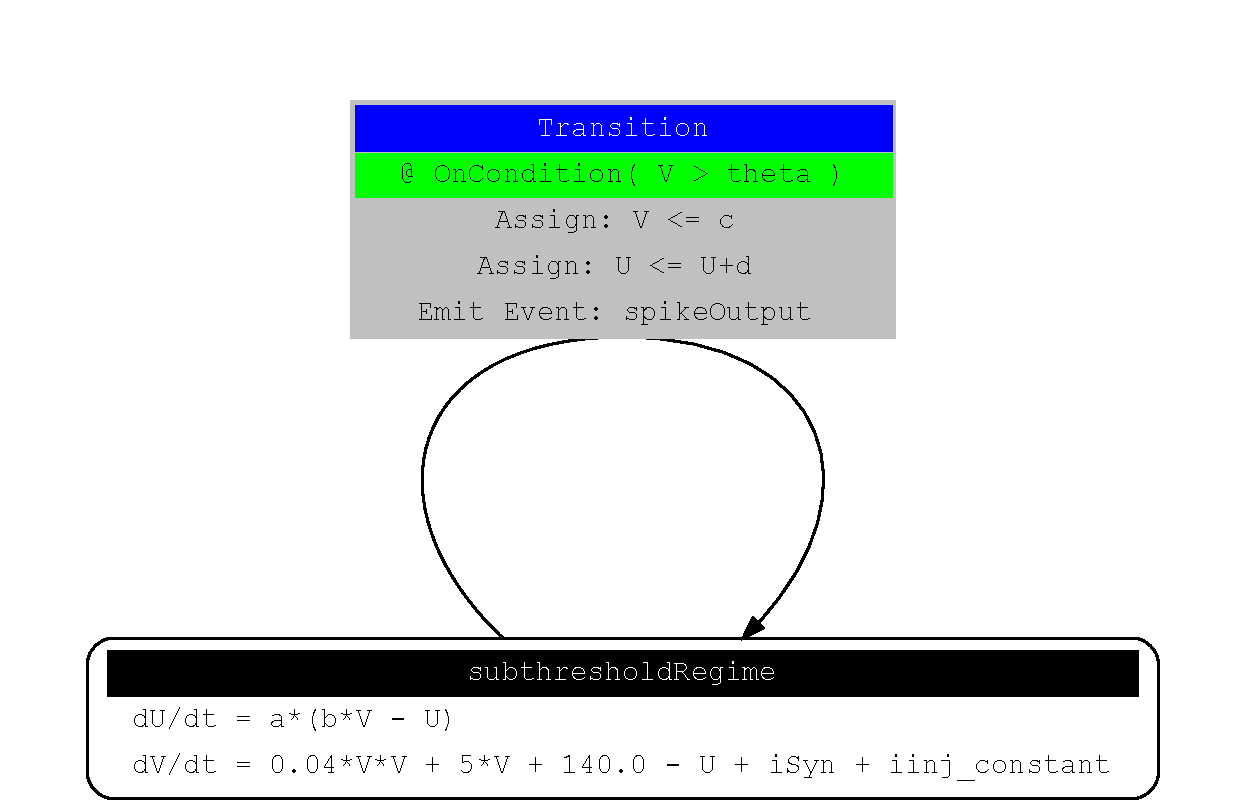
\includegraphics[width=8cm]{figures/example_IzRegimeTransGraph.pdf}
\protect\caption{{\tt RegimeGraph} for the XML model in this section.}
\label{fig:EX1_RegimeGraph}
\end{figure}

\noindent
Using this Abstraction Layer definition, as well as suitable parameters from the
user layer; $a=0.02, b=0.2, c=-65, d= 8, i_{\mathrm{injected}}= 5.0$, we can simulate
this, giving output as shown in Figure~\ref{fig:Ex1_Output}.

In Figure~\ref{fig:Ex1_Output}, we can see the value of the \StateVariable $V$
over time. We can also see that when the value of $V>theta$ triggers the
condition, we emit a spike, and the \StateAssignment of $V \leftarrow c$ resets
the value of $V$.
\clearpage
The corresponding Abstraction Layer XML description for this model is the following:
\begin{lstlisting}
<?xml version="1.0" encoding='UTF-8'?>
<NineML xmlns="http://nineml.net/9ML/1.0"
    xmlns:xsi="http://www.w3.org/2001/XMLSchema-instance"
    xsi:schemaLocation="http://nineml.net/9ML/1.0/NineML_v1.0.xsd">
  <ComponentClass name="IzhikevichCell">
    <Parameter name="a" dimension="dimensionless"/>
    <Parameter name="c" dimension="voltage"/>
    <Parameter name="b" dimension="per_time"/>
    <Parameter name="d" dimension="voltage_per_time"/>
    <Parameter name="theta" dimension="voltage"/>
    <Parameter name="i_injected" dimension="current"/>
    <AnalogReducePort name="i_synapse" operator="+" dimension="current"/>
    <AnalogSendPort name="U" dimension="dimensionless"/>
    <AnalogSendPort name="V" dimension="voltage"/>
    <EventPort name="spikeOutput" mode="send"/>
    <Dynamics>
        <StateVariable name="V" dimension="voltage"/>
        <StateVariable name="U" dimension="voltage_per_time"/>
        <Alias name="rv">
            <MathInline>V*U</MathInline>
        </Alias>
        <Regime name="subthresholdRegime">
          <TimeDerivative variable="U">
            <MathInline>a*(b*V - U)</MathInline>
          </TimeDerivative>
          <TimeDerivative variable="V">
            <MathInline>0.04*V*V + 5*V + 140.0 - U + i_synapse + i_injected</MathInline>
          </TimeDerivative>
          <OnCondition>
            <Trigger>
              <MathInline>V &gt; theta </MathInline>
            </Trigger>
            <StateAssignment variable="V" >
              <MathInline>c</MathInline>
            </StateAssignment>
            <StateAssignment variable="U" >
              <MathInline>U+d</MathInline>
            </StateAssignment>
            <EventOut port="spikeOutput" />
          </OnCondition>
        </Regime>
    </Dynamics>
  </ComponentClass>
  <Dimension name="per_time" t="-1"/>
  <Dimension name="voltage" m="1" l="2" t="-3" i="-1"/>
  <Dimension name="voltage_per_time" m="1" l="2" t="-4" i="-1"/>
  <Dimension name="current" i="1"/>
  <Dimension name="dimensionless"/>  
</NineML>
\end{lstlisting}

\clearpage
User Layer description for the above example:

\begin{lstlisting}
<?xml version='1.0' encoding='UTF-8'?>
<NineML xmlns="http://nineml.net/9ML/1.0"
    xmlns:xsi="http://www.w3.org/2001/XMLSchema-instance"
    xsi:schemaLocation="http://nineml.net/9ML/1.0/NineML_v1.0.xsd">
  <Component name="IzhikevichNeuron">
    <Definition url="http://nineml.net/catalog/izhikevichCell.9ml"
      >IzhikevichCell</Definition>
    <Property name="V" units="mV">
      <SingleValue>-60</SingleValue>
    </Property>
    <Property name="U" units="mV_per_ms">
      <SingleValue>0</SingleValue>
    </Property>
    <Property name="theta" units="mV">
      <SingleValue>50</SingleValue>
    </Property>
    <Property name="a" units="none">
      <SingleValue>0.02</SingleValue>
    </Property>
    <Property name="b" units="per_ms">
      <SingleValue>0.2</SingleValue>
    </Property>
    <Property name="c" units="mV">
      <SingleValue>-65</SingleValue>
    </Property>
    <Property name="d" units="mV_per_ms">
      <SingleValue>8</SingleValue>
    </Property>
  </Component>
  <Dimension name="per_time" t="-1"/>
  <Dimension name="voltage" m="1" l="2" t="-3" i="-1"/>
  <Dimension name="voltage_per_time" m="1" l="2" t="-4" i="-1"/>
  <Dimension name="current" i="1"/>
  <Dimension name="dimensionless"/>
  <Unit symbol="mV" dimension="voltage" power="-3" />
  <Unit symbol="per_ms" dimension="per_time" power="-3" />
  <Unit symbol="mV_per_ms" dimension="voltage_per_time" />
  <Unit symbol="none" dimension="dimensionless" />
</NineML>
\end{lstlisting}

Here, we show the simulation results of this XML representation.
\begin{figure}[htb!]
\center
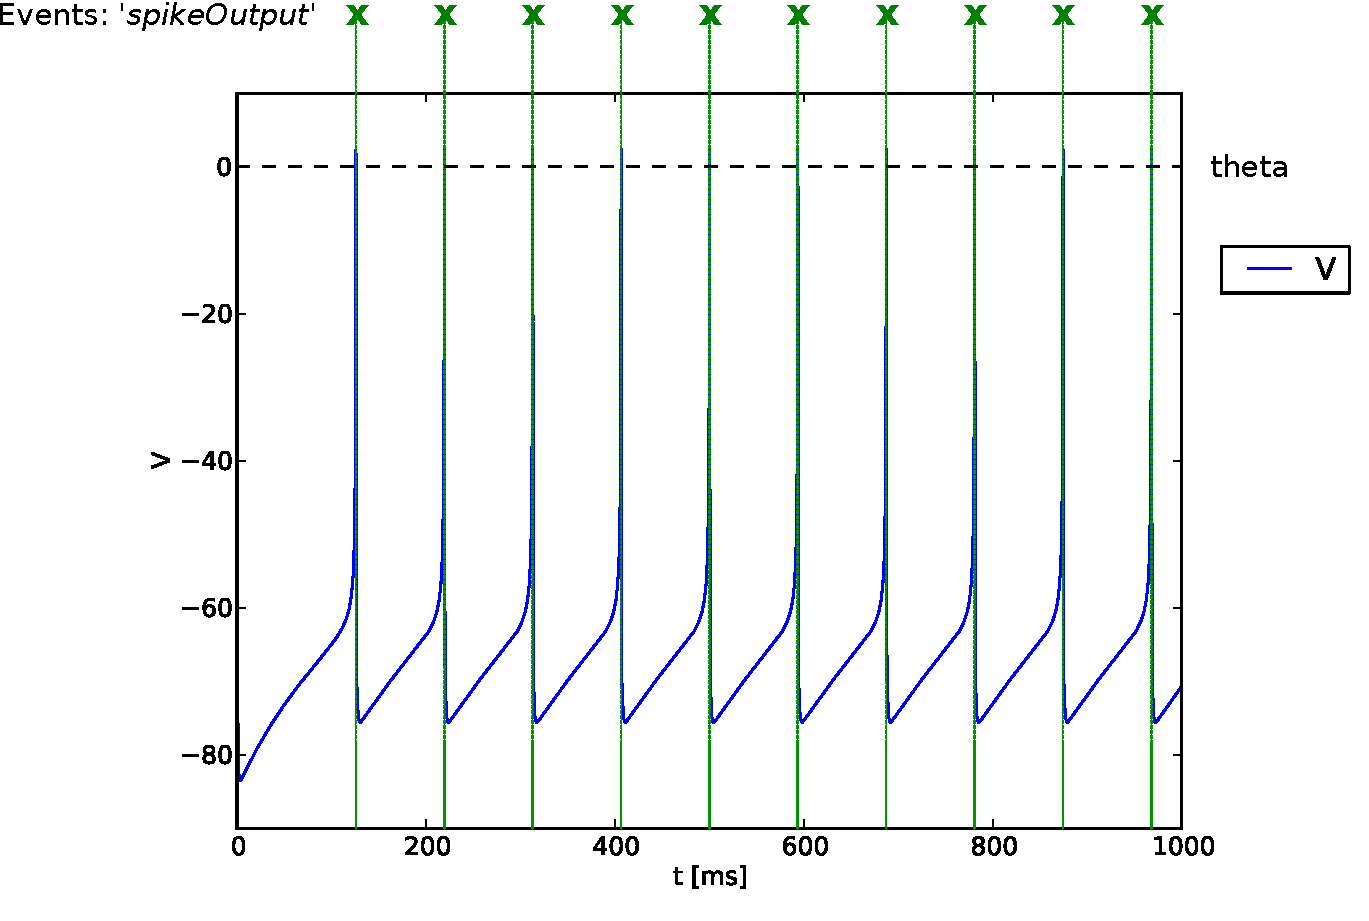
\includegraphics[width=8cm]{figures/example_IzVoltageWave.pdf}
\protect\caption{Result of simulating of the XML model in
this section}
\label{fig:Ex1_Output}
\end{figure}

\newpage
\subsection{Leaky Integrate and Fire model}

In this example, we build a representation of a integrate-and-fire neuron, with
an attached input synapse.
\noindent
We have a single \StateVariable, \emph{iaf\_V}.
This time, the neuron has an absolute refractory period; which is implemented
by using 2 regimes. \emph{RegularRegime} \& \emph{RefractoryRegime}
In \emph{RegularRegime}, the neuron voltage evolves as:
\begin{eqnarray}
\frac{d(iaf\_V)}{dt} = \frac{ iaf\_gl*( iaf\_vrest - iaf\_V ) + iaf\_ISyn+cobaExcit\_I} {iaf\_cm}
\end{eqnarray}
In \emph{RefractoryRegime}, the neuron voltage does not change in response to any
input:

\begin{eqnarray}
\frac{d(iaf\_V)}{dt} = 0
\end{eqnarray}
\noindent
In both Regimes, the synapses dynamics evolve as:
\begin{eqnarray}
\frac{d(cobaExcit\_g)}{dt} = - \frac{cobaExcit\_g}{cobaExcit\_tau}
\end{eqnarray}
\noindent
The neuron has 2 EventPorts, \emph{iaf\_spikeoutput} is a send port, which sends
events when the neuron fires, and \emph{cobaExcit\_spikeinput} is a recv port,
which tells the attached synapse that it should `fire'.
\noindent
The neuron has 4 transitions, 2 {\OnEvent} transitions  and 2 {\OnCondition} transitions.
Two of the Transitions are triggered by \emph{cobaExcit\_spikeinput} events, which
cause the conductance of the synapse to increase by an amount $q$, These
happen in both Regimes.
The other {\OnCondition}s:
\begin{itemize}
\item One is triggered the voltage being above threshold, which moves the
component from \emph{RegularRegime} to \emph{RefractoryRegime}, sets V to the
reset-voltage also emits a spike
\item The other is triggered by enough time having passed for the component
to come out of the \emph{RefractoryRegime} and move back to the \emph{RegularRegime}
\end{itemize}

The corresponding Regime Graph is shown in Figure 5.

\begin{figure}[htb!]
\center
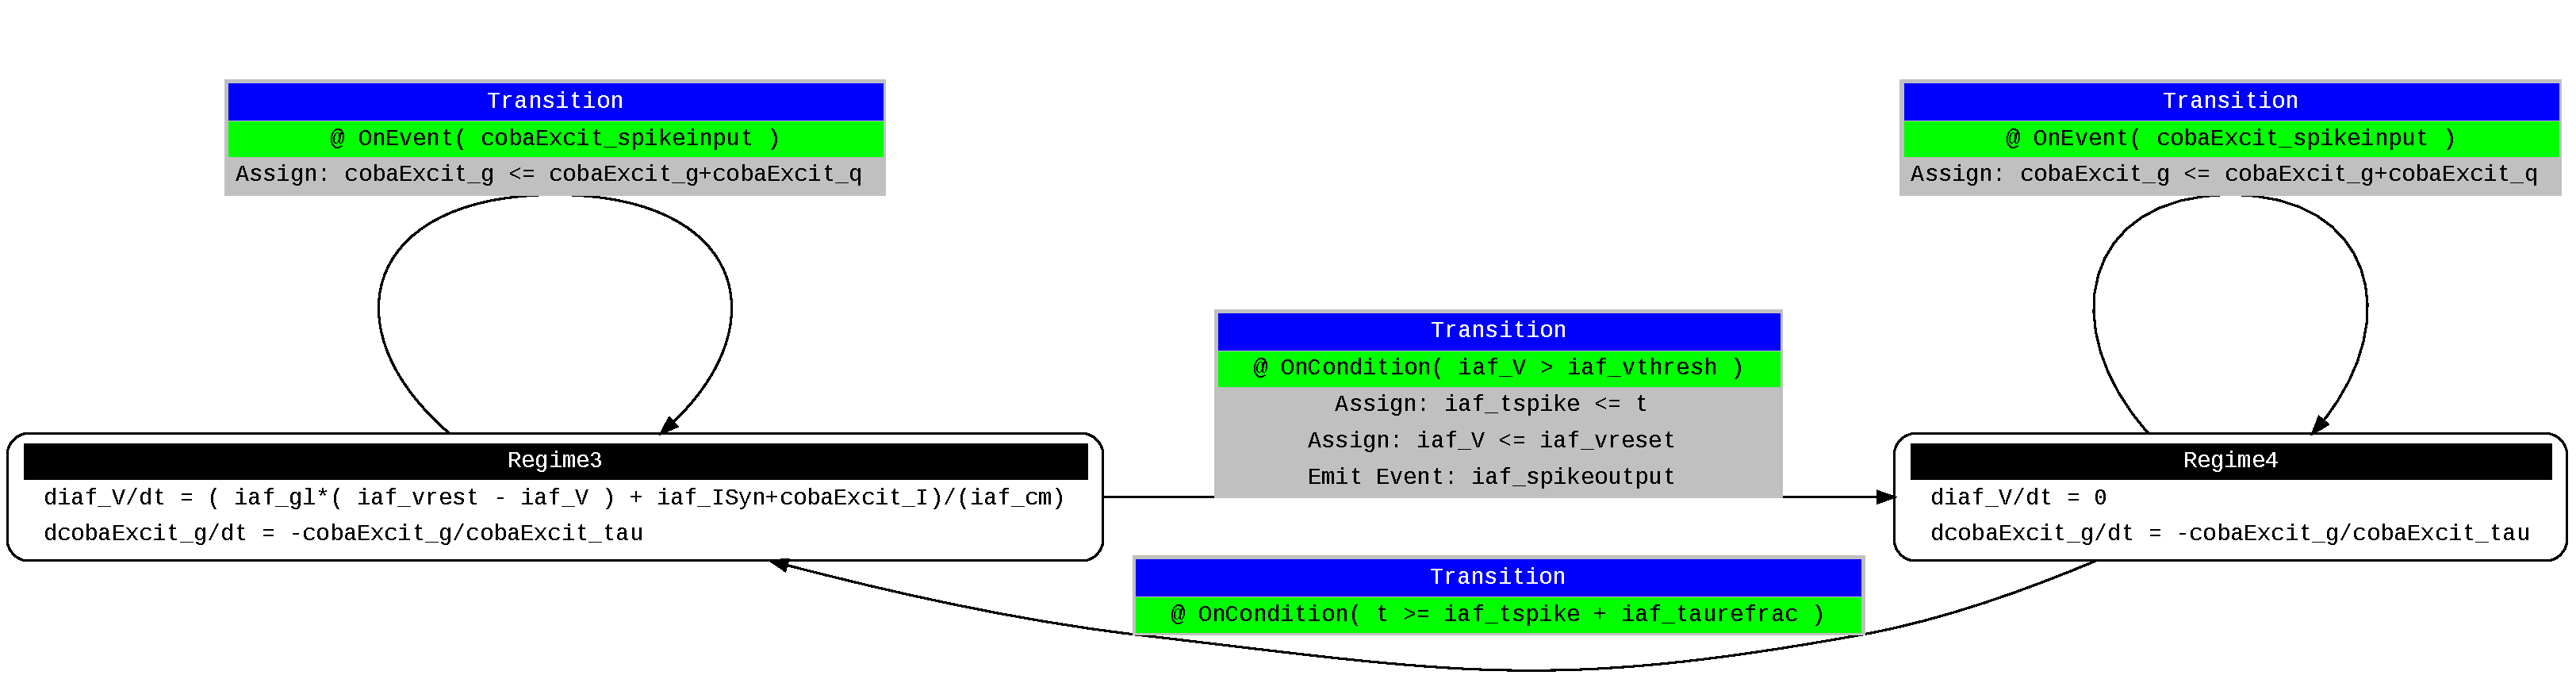
\includegraphics[width=14cm]{figures/demo2_Coba1_trnasition.pdf}
\protect\caption{RegimeGraph for the XML model in this section}
\label{fig:EX2_trans}
\end{figure}
\clearpage
The resulting XML description for the Abstraction Layer is :
\begin{lstlisting}[label=code:xmliaf2]
<?xml version='1.0' encoding='UTF-8'?>
<NineML xmlns="http://nineml.net/9ML/1.0">
  <ComponentClass name="Iaf1Coba">
    <AnalogSendPort dimension="voltage" name="iaf_V" />
    <AnalogReducePort dimension="current" operator="+" name="iaf_ISyn" />
    <AnalogSendPort dimension="current" name="cobaExcit_I" />
    <EventSendPort name="iaf_spikeoutput"/>
    <EventReceivePort name="cobaExcit_spikeinput"/>
    <Parameter dimension="area" name="iaf_cm"/>
    <Parameter dimension="time" name="iaf_taurefrac"/>
    <Parameter dimension="conductance" name="iaf_gl"/>
    <Parameter dimension="voltage" name="iaf_vreset"/>
    <Parameter dimension="voltage" name="iaf_vrest"/>
    <Parameter dimension="voltage" name="iaf_vthresh"/>
    <Parameter dimension="time" name="cobaExcit_tau"/>
    <Parameter dimension="conductance" name="cobaExcit_q"/>
    <Parameter dimension="voltage" name="cobaExcit_vrev"/>
    <Dynamics>
      <StateVariable dimension="voltage" name="iaf_V"/>
      <StateVariable dimension="time" name="iaf_tspike"/>
      <StateVariable dimension="conductance" name="cobaExcit_g"/>
      <Regime name="RefractoryRegime">
        <TimeDerivative variable="iaf_V">
          <MathInline>0</MathInline>
        </TimeDerivative>
        <TimeDerivative variable="cobaExcit_g">
          <MathInline>-cobaExcit_g/cobaExcit_tau</MathInline>
        </TimeDerivative>
        <OnEvent target_regime="RefractoryRegime" src_port="cobaExcit_spikeinput">
          <StateAssignment variable="cobaExcit_g">
            <MathInline>cobaExcit_g+cobaExcit_q</MathInline>
          </StateAssignment>
        </OnEvent>
        <OnCondition target_regime="RegularRegime">
          <Trigger>
            <MathInline>t &gt;= iaf_tspike + iaf_taurefrac</MathInline>
          </Trigger>
        </OnCondition>
      </Regime>
      <Regime name="RegularRegime">
        <TimeDerivative variable="iaf_V">
          <MathInline>( iaf_gl*( iaf_vrest - iaf_V ) + iaf_ISyn+cobaExcit_I)/(iaf_cm)</MathInline>
        </TimeDerivative>
        <TimeDerivative variable="cobaExcit_g">
          <MathInline>-cobaExcit_g/cobaExcit_tau</MathInline>
        </TimeDerivative>
        <OnEvent target_regime="RegularRegime" src_port="cobaExcit_spikeinput">
          <StateAssignment variable="cobaExcit_g">
            <MathInline>cobaExcit_g+cobaExcit_q</MathInline>
          </StateAssignment>
        </OnEvent>
        <OnCondition target_regime="RefractoryRegime">
          <StateAssignment variable="iaf_tspike">
            <MathInline>t</MathInline>
          </StateAssignment>
          <StateAssignment variable="iaf_V">
            <MathInline>iaf_vreset</MathInline>
          </StateAssignment>
          <EventOut port="iaf_spikeoutput"/>
          <Trigger>
            <MathInline>iaf_V &gt; iaf_vthresh</MathInline>
          </Trigger>
        </OnCondition>
      </Regime>
      <Alias name="cobaExcit_I">
        <MathInline>cobaExcit_g*(cobaExcit_vrev-iaf_V)</MathInline>
      </Alias>
    </Dynamics>
  </ComponentClass>
  <Dimension name="time" t="1"/>
  <Dimension name="voltage" m="1" l="2" t="-3" i="-1"/>
  <Dimension name="conductance" m="-1" t="3" l="-2" i="2"/>
  <Dimension name="area" l="2"/>
</NineML>
\end{lstlisting}

User Layer description for the above example:
\begin{lstlisting}
<?xml version='1.0' encoding='UTF-8'?>
<NineML xmlns="http://nineml.net/9ML/2.0">
  <Component name="IaFNeuron">
    <Definition url="http://nineml.net/catalog/neurons/iafICoba.9ml"
      >Iaf1Coba</Definition>
    <Property name="iaf_V" units="mV">
      <SingleValue>-60</SingleValue>
    </Property>
    <Property name="iaf_tspike" units="ms">
      <SingleValue>-1</SingleValue>
    </Property>
    <Property name="cobaExcit_g" units="mS">
      <SingleValue>0</SingleValue>
    </Property>
    <Property name="iaf_cm" units="cm_square">
      <SingleValue>0.02</SingleValue>
    </Property>
    <Property name="iaf_taurefrac" units="ms">
      <SingleValue>3</SingleValue>
    </Property>
    <Property name="iaf_gl" units="mS">
      <SingleValue>0.1</SingleValue>
    </Property>
    <Property name="iaf_vreset" units="mV">
      <SingleValue>-70</SingleValue>
    </Property>
    <Property name="iaf_vrest" units="mV">
      <SingleValue>-60</SingleValue>
    </Property>
    <Property name="iaf_vthresh" units="mV">
      <SingleValue>20</SingleValue>
    </Property>
    <Property name="cobaExcit_tau" units="ms">
      <SingleValue>2</SingleValue>
    </Property>
    <Property name="cobaExcit_q" units="ms">
      <SingleValue>1</SingleValue>
    </Property>
    <Property name="cobaExcit_vrev" units="mV">
      <SingleValue>0</SingleValue>
    </Property>
  </Component>
  <Dimension name="time" t="1"/>
  <Dimension name="voltage" m="1" l="2" t="-3" i="-1"/>
  <Dimension name="conductance" m="-1" t="3" l="-2" i="2"/>
  <Dimension name="area" l="2"/>
  <Unit symbol="mV" dimension="voltage" power="-3"/>
  <Unit symbol="ms" dimension="time" power="-3"/>
  <Unit symbol="cm_square" dimension="area" power="-4"/>
  <Unit symbol="mS" dimension="conductance" power="-3"/>
</NineML>
\end{lstlisting}

The simulation results is presented in Figure 6.
\begin{figure}[htb!]
\center
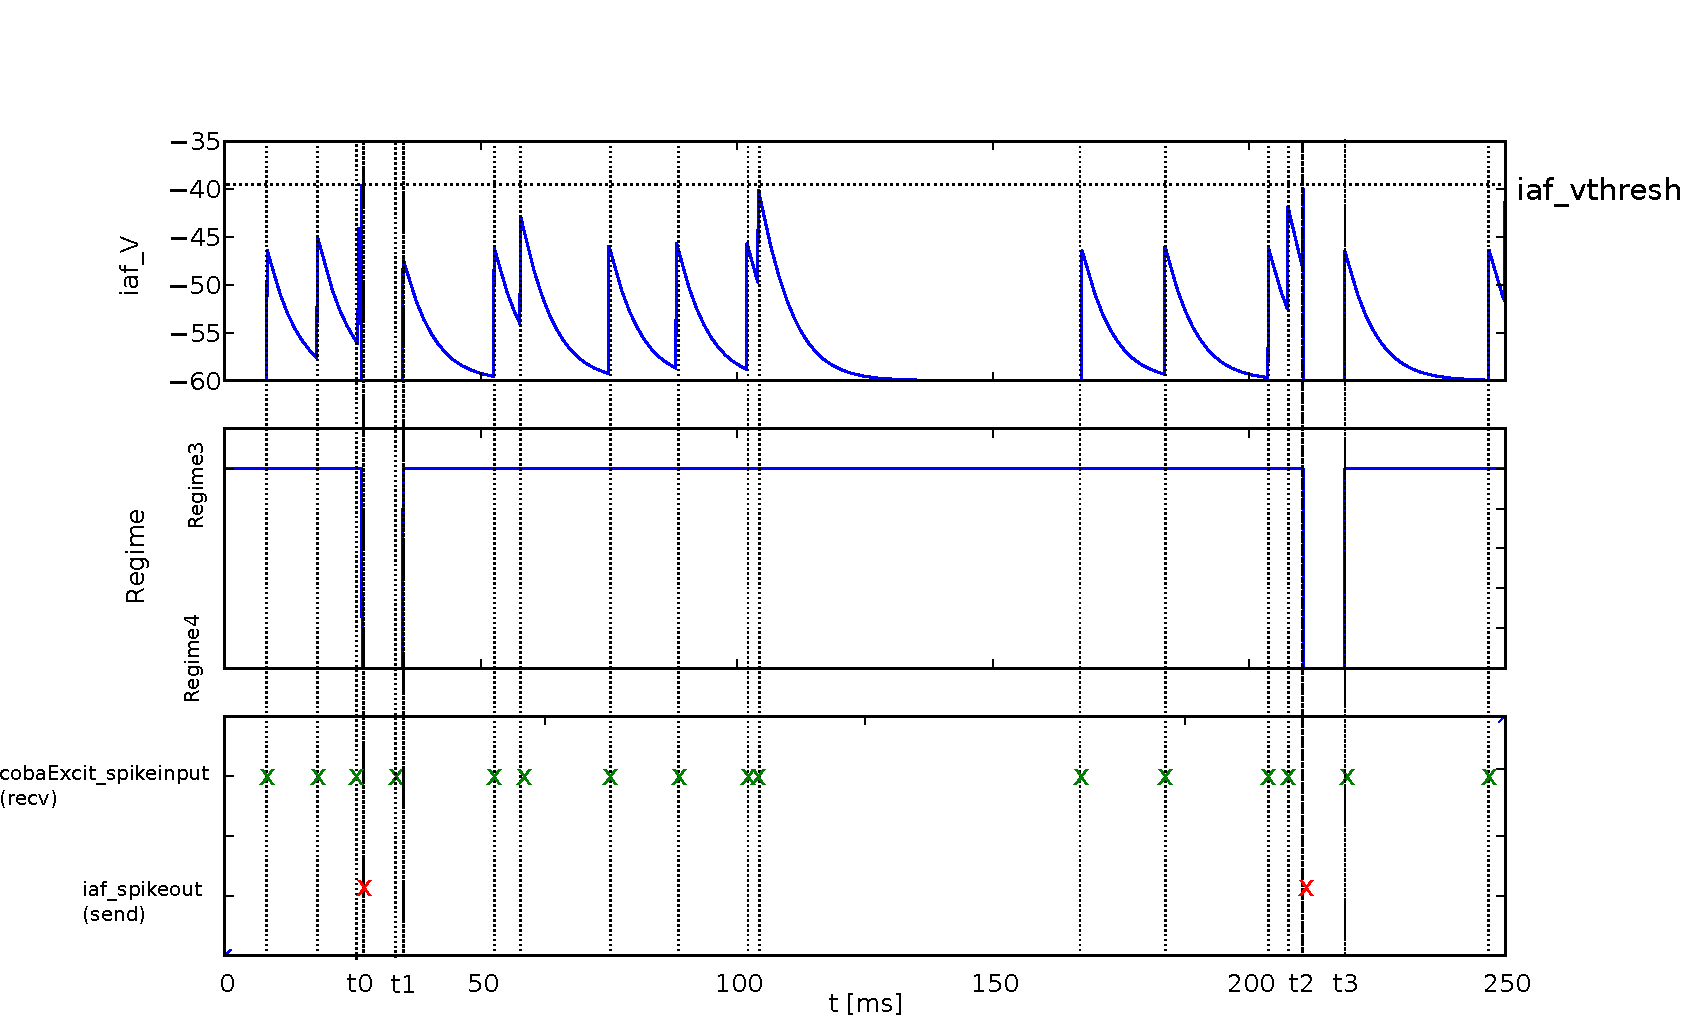
\includegraphics[width=14cm]{figures/demo2_Coba1_out.pdf}
\protect\caption{Result of simulating of the XML model in this section.
\emph{cobaExcit\_spikeinput} is fed events from an external Poisson generator
in this simulation}
\label{fig:EX2_Output}
\end{figure}

\clearpage
\subsection{Multi-component Hodgkin-Huxley Model}

\begin{lstlisting}
<?xml version="1.0" encoding="UTF-8"?>
<NineML xmlns="http://nineml.net/9ML/2.0">
  <MultiComponent name="HodgkinHuxleyContainer">
    <SubComponent name="Na">
      <Component>
        <Definition>PyramidalNa</Definition>
        <Property name="gbar" units="uS">
          <SingleValue>0.0025</SingleValue>
        </Property>
      </Component>
      <ReceiveConnection port="V">
        <FromSister component="membrane" port="V"/>
      </ReceiveConnection>
    </SubComponent>
    <SubComponent name="K">
      <Component>
        <Prototype>PyramidalK</Prototype>
        <Property name="gbar" units="uS">
          <SingleValue>0.0036</SingleValue>
        </Property>
      </Component>
      <ReceiveConnection port="V">
        <FromSister component="membrane" port="V"/>
      </ReceiveConnection>
    </SubComponent>
    <SubComponent name="leak">
      <Component>
        <Definition>Leak</Definition>
        <Property name="g" units="uS">
          <SingleValue>0.001</SingleValue>
        </Property>
        <Property name="e_rev" units="mV">
          <SingleValue>-21</SingleValue>
        </Property>
      </Component>
      <ReceiveConnection port="V">
        <FromSister component="membrane" port="V"/>
      </ReceiveConnection>
    </SubComponent>
    <SubComponent name="membrane">
      <Component>
        <Definition url="http://nineml.net/9ML/2.0/catalog/basicMembrane.9ml"
          >BasicMembrane</Definition>
        <Property name="length" units="um">
          <SingleValue>15.0</SingleValue>
        </Property>
        <Property name="axialResistance" units="ohm_per_cm">
          <SingleValue>100.0</SingleValue>
        </Property>
        <Property name="diameter" units="um">
          <SingleValue>15.0</SingleValue>
        </Property>
        <Property name="C" units="uF">
          <SingleValue>1.0</SingleValue>
        </Property>
      </Component>
      <ReceiveConnection port="i">
        <FromSister component="Na" name="i"/>
        <FromSister component="K" name="i"/>
        <FromSister component="leak" name="i"/>
      </ReceiveConnection>
    </SubComponent>
    <PortExposure name="membraneVoltage" component="membrane" port="V"/>
    <PortExposure name="membraneCurrent" component="membrane" port="i">
      <Annotations>
        <Comment>This can be used to connect current synaptic input</Comment>
      </Annotations>
    </PortExposure>
  </MultiComponent>
  <Dimension name="time" t="1"/>
  <Dimension name="voltage" m="1" l="2" t="-3" i="-1"/>
  <Dimension name="conductance" m="-1" t="3" l="-2" i="2"/>
  <Dimension name="area" l="2"/>
  <Dimension name="length" l="1"/>
  <Unit symbol="mV" dimension="voltage" power="-3"/>
  <Unit symbol="um" dimension="length" power="-6"/>
  <Unit symbol="ms" dimension="time" power="-3"/>
  <Unit symbol="cm_square" dimension="area" power="-4"/>
  <Unit symbol="mS" dimension="conductance" power="-3"/>  
</NineML>\end{lstlisting}

\clearpage
\subsection{Example multi-compartmental model}

\begin{lstlisting}
<?xml version="1.0" encoding="UTF-8"?>
<NineML xmlns="http://nineml.net/9ML/2.0">
  <MultiCompartmental name="ExampleMultiCompartmentModel">
    <Definition>ExampleMultiCompartmentClass</Definition>
    <Branches>
      <ExternalArrayValue url="./example_compartments.txt"
        mimetype="vnd.net.nineml.arrayvalue.text" columnName="parentID"/>
    </Branches>
    <Mapping>
      <ExternalArrayValue url="./example_compartments.txt"
        mimetype="vnd.net.nineml.arrayvalue.text" columnName="domain"/>
    </Mapping>
    <Domain name="soma">
      <MultiComponent name="somaDynamics">
        <SubComponent name="PyramidalNa">
          <Component>
            <Prototype url="http://nineml.net/9ML/2.0/catalog/channels"
              >HHPyramidalNa</Prototype>
            <Property name="gbar" units="uS">
              <SingleValue>0.0036</SingleValue>
            </Property>
          </Component>
          <ReceiveConnection port="V">
            <FromSister component="membrane" port="V"/>
          </ReceiveConnection>
        </SubComponent>
        <SubComponent name="PyramidalK">
          <Component>
            <Prototype url="http://nineml.net/9ML/2.0/catalog/channels"
              >HHPyramidalK</Prototype>
            <Property name="gbar" units="uS">
              <SingleValue>0.0025</SingleValue>
            </Property>
          </Component>
          <ReceiveConnection port="V">
            <FromSister component="membrane" port="V"/>
          </ReceiveConnection>
        </SubComponent>
        <SubComponent name="Kv4">
          <Component>
            <Prototype url="http://nineml.net/9ML/2.0/catalog/channels"
              >HHPyramidalK</Prototype>
            <Property name="gbar" units="uS">
              <SingleValue>0.0025</SingleValue>
            </Property>
          </Component>
          <ReceiveConnection port="V">
            <FromSister component="membrane" port="V"/>
          </ReceiveConnection>
        </SubComponent>
        <SubComponent name="leak">
          <Component>
            <Definition url="http://nineml.net/9ML/2.0/catalog/channels"
              >Leak</Definition>
            <Property name="g" units="uS">
              <SingleValue>0.001</SingleValue>
            </Property>
            <Property name="e_rev" units="mV">
              <SingleValue>-21</SingleValue>
            </Property>
          </Component>
          <ReceiveConnection port="V">
            <FromSister component="membrane" port="V"/>
          </ReceiveConnection>
        </SubComponent>
        <SubComponent name="membrane">
          <Component>
            <Definition url="http://nineml.net/9ML/2.0/catalog/channels/basicCompartment.9ml"
              >BasicCompartment</Definition>
            <Property name="length" units="um">
              <SingleValue>15.0</SingleValue>
            </Property>
            <Property name="axialResistance" units="ohm_per_cm">
              <SingleValue>100.0</SingleValue>
            </Property>
            <Property name="diameter" units="um">
              <SingleValue>15.0</SingleValue>
            </Property>
            <Property name="C" units="uF">
              <SingleValue>1.0</SingleValue>
            </Property>
          </Component>
          <ReceiveConnection port="i">
            <FromSister component="Na" name="i"/>
            <FromSister component="K" name="i"/>
            <FromSister component="leak" name="i"/>
          </ReceiveConnection>
        </SubComponent>
        <PortExposure name="proximalVoltage" component="membrane" port="proximalV"/>
        <PortExposure name="distalVoltage" component="membrane" port="distalV"/>
      </MultiComponent>
      <ReceiveConnection port="proximalVoltage">
        <FromProximal port="voltage"/>
      </ReceiveConnection>
      <ReceiveConnection port="distalVoltage">
        <FromDistal port="voltage"/>
      </ReceiveConnection>
    </Domain>
    <Domain name="dendrites">
      <Reference>DendriteDynamics</Reference>
      <ReceiveConnection port="proximalVoltage">
        <FromProximal port="voltage"/>
      </ReceiveConnection>
      <ReceiveConnection port="distalVoltage">
        <FromDistal port="voltage"/>
      </ReceiveConnection>
      <ReceiveConnection port="withinDendritesReducePort">
        <FromProximal domain="dendrites" port="withinDendritesSendPort"/>
        <FromDistal domain="dendrites" port="withinDendritesSendPort"/>
      </ReceiveConnection>
    </Domain>
    <Annotations>
      <Points3D>
        <XCoords>
          <ExternalArrayValue url="./example_compartments.txt.txt"
            mimetype="vnd.net.nineml.arrayvalue.text" columnName="X"/>
        </XCoords>
        <YCoords>
          <ExternalArrayValue url="./example_compartments.txt.txt"
            mimetype="vnd.net.nineml.arrayvalue.text" columnName="Y"/>
        </YCoords>
        <ZCoords>
          <ExternalArrayValue url="./example_compartments.txt.txt"
            mimetype="vnd.net.nineml.arrayvalue.text" columnName="Z"/>
        </ZCoords>
      </Points3D>
    </Annotations>
  </MultiCompartmental>
  <Dimension name="time" t="1"/>
  <Dimension name="voltage" m="1" l="2" t="-3" i="-1"/>
  <Dimension name="conductance" m="-1" t="3" l="-2" i="2"/>
  <Dimension name="area" l="2"/>
  <Dimension name="length" l="1"/>
  <Unit symbol="mV" dimension="voltage" power="-3"/>
  <Unit symbol="um" dimension="length" power="-6"/>
  <Unit symbol="ms" dimension="time" power="-3"/>
  <Unit symbol="cm_square" dimension="area" power="-4"/>
  <Unit symbol="mS" dimension="conductance" power="-3"/>
</NineML>
\end{lstlisting}

\pagebreak

\newpage

\section{Transition resolution}
\label{resolution}

\draftnote{Do we really want to include this here? Transitions (with the exception of those which just emit spikes) should really be wound back to the exact time point in my opinion because handling multiple simultaneous (in terms of time steps) transitions doesn't seem well defined to me.}
This section outlines pseudo code which defines the order of
transition-triggering, state assignment execution, event emission,
transmission and resolution in a system of connected components.
Implementations do not need to implement this algorithm but should produce
the same behaviours.

A {\tt TransitionResolutionBlock} represents an instant in time. It begins
before any transitions occur and ends after each component has moved
into its new \Regime, all \textbf{StateAssignments} have been executed
and all Events generated and resolved in the system.

\subsection{Serial implementation of transition resolution}

\newcommand{\CN}[0]{\textsl{C\_n}}

We have a system of \textsl{N} components \textsl{\{C\_1,C\_2,...,C\_N\}},
at time, \textsl{t}, where each component, \CN, is in \Regime
$R^{t}_{n}$.

\noindent From \Regime $R^{t}_{n}$, there are:
\begin{itemize}
\item OnEvent transitions $OnEv^{t}_{n} = \{ ... \}$
\item OnCondition transitions $OnCond^{t}_{n} = \{ ... \}$
\end{itemize}

\newcommand{\send}[0]{\texttt{send} }
\newcommand{\recv}[0]{\texttt{recv} }

\noindent Component \CN
has:
\begin{itemize}
\item \send EventPorts \textsl{EvSend = \{$EvSend_{n,1,}$, $EvSend_{n,2,}$, ... \}}
\item \recv EventPorts \textsl{EvRecv = \{$EvRecv_{n,1,}$, $EvRecv_{n,2,}$, ... \}}
\end{itemize}

\noindent EventPort connections are stored in a a map,
\textsl{EvPortConnections}, which maps EvSend to a list of EvRecv ports. i.e.,

\textsl{\{EvSend $\rightarrow$ [EvRecv,EvRecv,..,EvRecv], EvSend $\rightarrow$
[EvRecv,EvRecv,EvRecv,...,EvRecv]\}}.

\newcommand{\RCLn}{$RCL_n$}
\newcommand{\AUTQn}{$AUTQ_n$}
\newcommand{\EQn}{$EQ_n$}

\noindent Each component has 3 associated data structures
\begin{itemize}
\item RegimeChangeList (\RCLn) (This list will contain target-regimes of
triggered transitions)
\item ActiveUnresolvedTransitionsQueue (\AUTQn) (This queue will
contain transitions which will occur, but their effects have not be
evaluated yet)
\item EventQueue (\EQn) (This list contains events delivered to this
component from other components via EventPort-connections)
\end{itemize}

\subsubsection{Algorithm}

\begin{enumerate}
\item Enter {\tt TransitionResolutionBlock}
\item For each component, \CN: clear \RCLn, \AUTQn and \EQn.
\item For each component, \CN: for each \textsl{oncond} in $OnCond^{t}_{n}$ : if
\textsl{oncond.trigger} evaluates to true, add \textsl{oncond} to \AUTQn.
\item For each component, \CN:  for each \textsl{tr} in \AUTQn :
\begin{itemize}
\item
remove \textsl{tr} from \AUTQn
\item add the target\_regime to \RCLn
\item for each
\textsl{action} in \textsl{tr.do}:
\begin{itemize}
\item if \textsl{action} is an OutputEvent: test
if the OutputEvent port is a key in \textsl{EvPortConnections}. If so, add the
    OutputEvent to the EventQueue (\textsl{EQ\_{target}}) corresponding to each
    \textsl{EvRecv} in the \textsl{EvPortConnections} map.

\item  if \textsl{action}  is a StateAssignment, execute that state-assignment
immediately.
\end{itemize}
\end{itemize}

\item For each component \CN: for each event, \textsl{EvRecv} in \EQn: test
whether there is a transition, \textsl{tr} triggered by this event, i.e an
OnEvent in $OnEv^t_n$ from $R^t_n$ ; if so; then add it to \AUTQn.

\item While any component has a non-empty \textsl{AUTQ}: Goto (4).

\item For each component, \CN, check that all the target-regimes in the \RCLn
are the same regime. (If not raise a RuntimeError). Each component moves into
this target-regime, or remains in the same regime if \RCLn is empty.

\item Leave {\tt TransitionResolutionBlock}

\end{enumerate}

\subsubsection{Notes}

\begin{enumerate}
\item \draftnote{Not sure about this either. Since a transition can also mean transitioning to a new regime it would
be very bad if two conditions were met at the same time and it was ambiguous which was applied first. Should
we not require an order of execution if there are multiple {\OnCondition}s in the same regime. Could be quite difficult
for the user to handle this otherwise}
There is no order defined in transitions; this means
that the order of resolution of state assignments can be ambiguous. If, for
example, we have two transitions, T1 and T2, originating from the same \Regime,
in which T1 contains the state assignment \textsl{V=V+1} and T2 contains the
assignment \textsl{V=V*V}, and both transitions are triggered simultaneously, then there is no
guarantee about the value of V. It is up the user to ensure this does not
happen.

\draftnote{I am not sure this is a good idea, we could just not allow \EventOut in \OnEvent transitions}
\item This Resolution System allows \emph{cascading} of Events, which in theory
could be recursive through components, depending on connectivity. The
implementation allows for this; and it is the users responsibility to ensure
that there are not such issues. The implementation may decided to terminate
Step (6) after a given number (say 1000) of iterations to prevent infinite
loops.

\end{enumerate}

\subsection{Parallelising of event resolution}

This algorithm can be parallelised as following. We create a thread for each
Component, which can independently execute Steps (3 to 6). The threads need
to be synchronized after steps (4) and (5) as shown in
Figure~\ref{ParallelisingTransitions}.

\begin{figure}[htb!]
\center
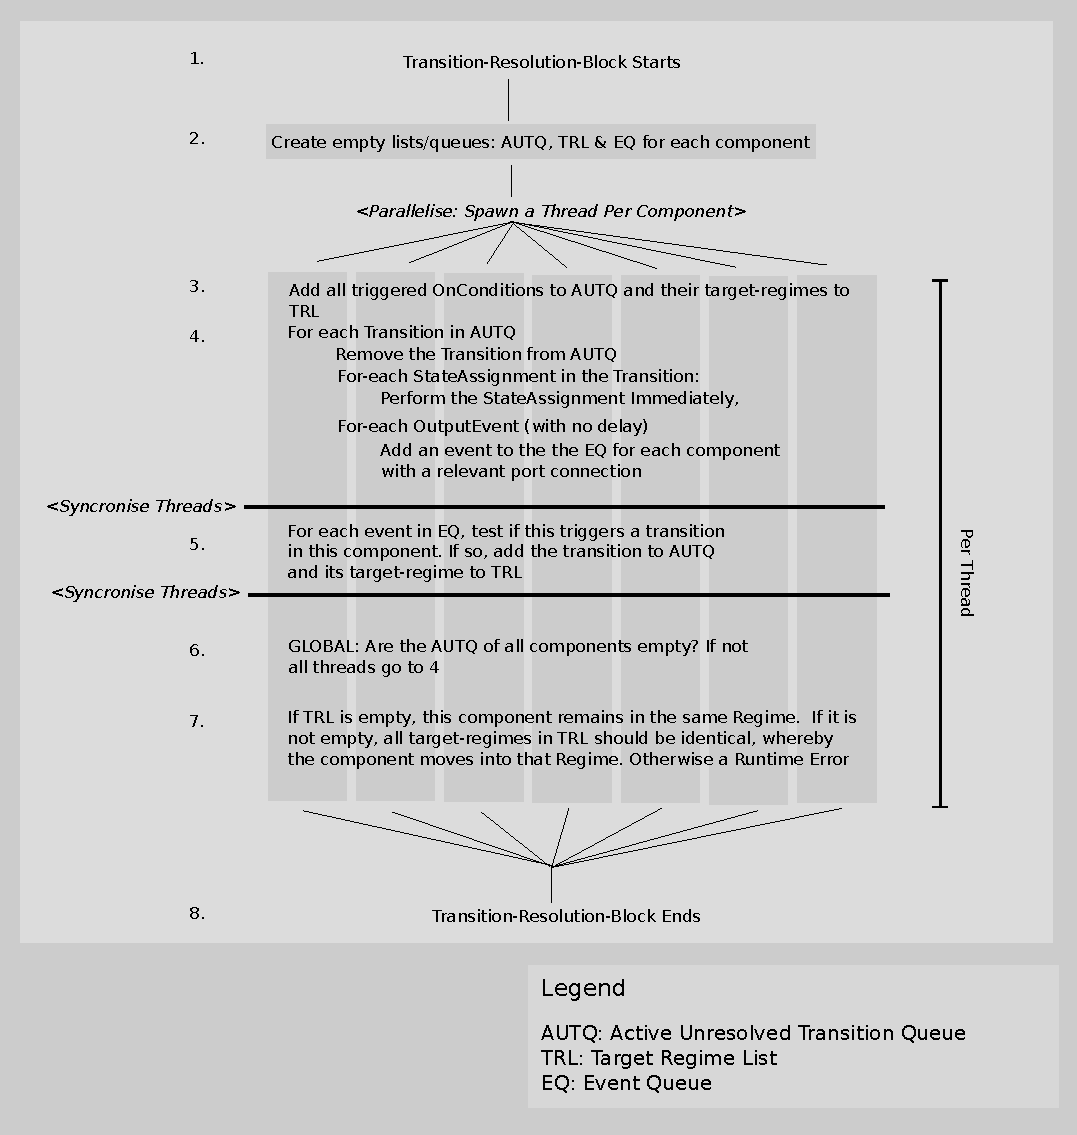
\includegraphics[width=14cm]{images/ParallelisingTransitions.pdf}
\protect\caption{Parallelising of Event Resolution.}
\label{ParallelisingTransitions}
\end{figure}

\section{Reserved Identifiers}
\label{sec:reserved_keywords}

In addition to the built-in mathematical functions and symbols (see \MathInline), the following strings (and capitalised versions) are reserved and cannot be used as identifiers,

\begin{multicols}{4}
\begin{itemize}
\item abs
\item abstract
\item alias
\item alignas
\item alignof
\item all
\item and
\item and\_eq
\item any
\item apply
\item arguments
\item as
\item asm
\item assert
\item auto
\item base
\item basestring
\item begin
\item bin
\item bitand
\item bitor
\item bool
\item boolean
\item break
\item buffer
\item byte
\item bytearray
\item callable
\item calloc
\item case
\item catch
\item char
\item char16\_t
\item char32\_t
\item checked
\item chr
\item class
\item classdef
\item classmethod
\item cmp
\item coerce
\item compile
\item compl
\item complex
\item const
\item const\_cast
\item constexpr
\item continue
\item debugger
\item decimal
\item decltype
\item def
\item default
\item del
\item delattr
\item delegate
\item delete
\item dict
\item dir
\item divmod
\item do
\item double
\item dynamic\_cast
\item elif
\item else
\item elseif
\item elsif
\item end
\item ensure
\item enum
\item enumerate
\item eval
\item event
\item except
\item exec
\item execfile
\item explicit
\item export
\item extends
\item extern
\item false
\item file
\item filter
\item final
\item finally
\item fixed
\item float
\item for
\item foreach
\item format
\item free
\item friend
\item from
\item frozenset
\item function
\item getattr
\item global
\item globals
\item goto
\item hasattr
\item hash
\item help
\item hex
\item id
\item if
\item implements
\item implicit
\item import
\item in
\item inline
\item input
\item instanceof
\item int
\item interface
\item intern
\item internal
\item is
\item isinstance
\item issubclass
\item iter
\item lambda
\item len
\item let
\item list
\item locals
\item lock
\item long
\item malloc
\item map
\item max
\item memchr
\item memcmp
\item memcpy
\item memmove
\item memoryview
\item memset
\item min
\item module
\item mutable
\item namespace
\item native
\item new
\item next
\item nil
\item noexcept
\item not
\item not\_eq
\item null
\item nullptr
\item object
\item oct
\item open
\item operator
\item or
\item or\_eq
\item ord
\item otherwise
\item out
\item override
\item package
\item params
\item parfor
\item pass
\item persistent
\item pow
\item print
\item private
\item property
\item protected
\item public
\item raise
\item range
\item raw\_input
\item readonly
\item realloc
\item redo
\item reduce
\item ref
\item register
\item reinterpret\_cast
\item reload
\item repr
\item rescue
\item retry
\item return
\item reversed
\item round
\item sbyte
\item sealed
\item self
\item set
\item setattr
\item short
\item signed
\item sizeof
\item slice
\item sorted
\item spmd
\item stackalloc
\item static
\item static\_assert
\item static\_cast
\item staticmethod
\item str
\item strictfp
\item string
\item struct
\item sum
\item super
\item switch
\item synchronized
\item template
\item then
\item this
\item thread\_local
\item throw
\item throws
\item transient
\item true
\item try
\item tuple
\item type
\item typedef
\item typeid
\item typename
\item typeof
\item uint
\item ulong
\item unchecked
\item undef
\item unichr
\item unicode
\item union
\item unless
\item unsafe
\item unsigned
\item until
\item ushort
\item using
\item var
\item vars
\item virtual
\item void
\item volatile
\item wchar\_t
\item when
\item while
\item with
\item xor
\item xor\_eq
\item xrange
\item yield
\item zip
\end{itemize}
\end{multicols}


\section{Acknowledgments}
\subsection{Former NineML INCF Task Force members}
\begin{itemize}
\item Abigail Morrison
\item Alex Cope
\item Anatoli Gorchetchnikov
\item Andrew P. Davison
\item Birgit Kriener
\item Chung-Chuan Lo
\item Damien Drix
\item Dragan Nikolic
\item Eilif Muller
\item Erik De Schutter
\item Hans Ekkehard Plesser
\item Hugo Cornelis
\item Ivan Raikov
\item Lars Schwabe
\item Malin Sandström
\item Michael Hull
\item Mikael Djurfeldt
\item Padraig Gleeson
\item Raphael Ritz
\item Robert Cannon
\item Robert Clewley
\item Sean Hill
\item Subhasis Ray
\item Valentin Haenel
\item Yann Le Franc
\end{itemize}

\clearpage
\bibliography{specification}

% -----------------------------------------------------------------------------
% End of document
% -----------------------------------------------------------------------------

\end{document}
